\documentclass[twoside]{book}

% Packages required by doxygen
\usepackage{fixltx2e}
\usepackage{calc}
\usepackage{doxygen}
\usepackage[export]{adjustbox} % also loads graphicx
\usepackage{graphicx}
\usepackage[utf8]{inputenc}
\usepackage{makeidx}
\usepackage{multicol}
\usepackage{multirow}
\PassOptionsToPackage{warn}{textcomp}
\usepackage{textcomp}
\usepackage[nointegrals]{wasysym}
\usepackage[table]{xcolor}

% Font selection
\usepackage[T1]{fontenc}
\usepackage[scaled=.90]{helvet}
\usepackage{courier}
\usepackage{amssymb}
\usepackage{sectsty}
\renewcommand{\familydefault}{\sfdefault}
\allsectionsfont{%
  \fontseries{bc}\selectfont%
  \color{darkgray}%
}
\renewcommand{\DoxyLabelFont}{%
  \fontseries{bc}\selectfont%
  \color{darkgray}%
}
\newcommand{\+}{\discretionary{\mbox{\scriptsize$\hookleftarrow$}}{}{}}

% Page & text layout
\usepackage{geometry}
\geometry{%
  a4paper,%
  top=2.5cm,%
  bottom=2.5cm,%
  left=2.5cm,%
  right=2.5cm%
}
\tolerance=750
\hfuzz=15pt
\hbadness=750
\setlength{\emergencystretch}{15pt}
\setlength{\parindent}{0cm}
\setlength{\parskip}{3ex plus 2ex minus 2ex}
\makeatletter
\renewcommand{\paragraph}{%
  \@startsection{paragraph}{4}{0ex}{-1.0ex}{1.0ex}{%
    \normalfont\normalsize\bfseries\SS@parafont%
  }%
}
\renewcommand{\subparagraph}{%
  \@startsection{subparagraph}{5}{0ex}{-1.0ex}{1.0ex}{%
    \normalfont\normalsize\bfseries\SS@subparafont%
  }%
}
\makeatother

% Headers & footers
\usepackage{fancyhdr}
\pagestyle{fancyplain}
\fancyhead[LE]{\fancyplain{}{\bfseries\thepage}}
\fancyhead[CE]{\fancyplain{}{}}
\fancyhead[RE]{\fancyplain{}{\bfseries\leftmark}}
\fancyhead[LO]{\fancyplain{}{\bfseries\rightmark}}
\fancyhead[CO]{\fancyplain{}{}}
\fancyhead[RO]{\fancyplain{}{\bfseries\thepage}}
\fancyfoot[LE]{\fancyplain{}{}}
\fancyfoot[CE]{\fancyplain{}{}}
\fancyfoot[RE]{\fancyplain{}{\bfseries\scriptsize Generated by Doxygen }}
\fancyfoot[LO]{\fancyplain{}{\bfseries\scriptsize Generated by Doxygen }}
\fancyfoot[CO]{\fancyplain{}{}}
\fancyfoot[RO]{\fancyplain{}{}}
\renewcommand{\footrulewidth}{0.4pt}
\renewcommand{\chaptermark}[1]{%
  \markboth{#1}{}%
}
\renewcommand{\sectionmark}[1]{%
  \markright{\thesection\ #1}%
}

% Indices & bibliography
\usepackage{natbib}
\usepackage[titles]{tocloft}
\setcounter{tocdepth}{3}
\setcounter{secnumdepth}{5}
\makeindex

% Hyperlinks (required, but should be loaded last)
\usepackage{ifpdf}
\ifpdf
  \usepackage[pdftex,pagebackref=true]{hyperref}
\else
  \usepackage[ps2pdf,pagebackref=true]{hyperref}
\fi
\hypersetup{%
  colorlinks=true,%
  linkcolor=blue,%
  citecolor=blue,%
  unicode%
}

% Custom commands
\newcommand{\clearemptydoublepage}{%
  \newpage{\pagestyle{empty}\cleardoublepage}%
}

\usepackage{caption}
\captionsetup{labelsep=space,justification=centering,font={bf},singlelinecheck=off,skip=4pt,position=top}

%===== C O N T E N T S =====

\begin{document}

% Titlepage & ToC
\hypersetup{pageanchor=false,
             bookmarksnumbered=true,
             pdfencoding=unicode
            }
\pagenumbering{alph}
\begin{titlepage}
\vspace*{7cm}
\begin{center}%
{\Large My Project }\\
\vspace*{1cm}
{\large Generated by Doxygen 1.8.13}\\
\end{center}
\end{titlepage}
\clearemptydoublepage
\pagenumbering{roman}
\tableofcontents
\clearemptydoublepage
\pagenumbering{arabic}
\hypersetup{pageanchor=true}

%--- Begin generated contents ---
\chapter{Class Index}
\section{Class List}
Here are the classes, structs, unions and interfaces with brief descriptions\+:\begin{DoxyCompactList}
\item\contentsline{section}{\hyperlink{structCounterexample}{Counterexample} \\*\hyperlink{structCounterexample}{Counterexample} struct to encode counterexamples }{\pageref{structCounterexample}}{}
\item\contentsline{section}{\hyperlink{classGame}{Game} }{\pageref{classGame}}{}
\item\contentsline{section}{\hyperlink{classParser}{Parser} }{\pageref{classParser}}{}
\end{DoxyCompactList}

\chapter{File Index}
\section{File List}
Here is a list of all documented files with brief descriptions\+:\begin{DoxyCompactList}
\item\contentsline{section}{\hyperlink{game_8h}{game.\+h} }{\pageref{game_8h}}{}
\item\contentsline{section}{\hyperlink{main_8cpp}{main.\+cpp} }{\pageref{main_8cpp}}{}
\item\contentsline{section}{\hyperlink{parserObject_8h}{parser\+Object.\+h} }{\pageref{parserObject_8h}}{}
\item\contentsline{section}{\hyperlink{teacher_8h}{teacher.\+h} }{\pageref{teacher_8h}}{}
\end{DoxyCompactList}

\chapter{Class Documentation}
\hypertarget{structCounterexample}{}\section{Counterexample Struct Reference}
\label{structCounterexample}\index{Counterexample@{Counterexample}}


\hyperlink{structCounterexample}{Counterexample} struct to encode counterexamples.  


\subsection*{Public Member Functions}
\begin{DoxyCompactItemize}
\item 
\mbox{\Hypertarget{structCounterexample_ad61919a508b1ea11f1182a25b2b1185e}\label{structCounterexample_ad61919a508b1ea11f1182a25b2b1185e}} 
{\bfseries Counterexample} (std\+::vector$<$ int $>$ \&dp, int c)
\end{DoxyCompactItemize}
\subsection*{Public Attributes}
\begin{DoxyCompactItemize}
\item 
\mbox{\Hypertarget{structCounterexample_a15f4bdb9016776361e63a942b200a637}\label{structCounterexample_a15f4bdb9016776361e63a942b200a637}} 
std\+::vector$<$ int $>$ {\bfseries datapoints}
\item 
\mbox{\Hypertarget{structCounterexample_ab79272d7c597224446a206a1abf5ac74}\label{structCounterexample_ab79272d7c597224446a206a1abf5ac74}} 
int {\bfseries classification}
\end{DoxyCompactItemize}
\subsection*{Friends}
\begin{DoxyCompactItemize}
\item 
\mbox{\Hypertarget{structCounterexample_a8af9efd24afb9650e8b336d5c8cf6770}\label{structCounterexample_a8af9efd24afb9650e8b336d5c8cf6770}} 
bool {\bfseries operator==} (const \hyperlink{structCounterexample}{Counterexample} \&c1, const \hyperlink{structCounterexample}{Counterexample} \&c2)
\item 
\mbox{\Hypertarget{structCounterexample_af264b295905bfbfe1438c52333c66e2b}\label{structCounterexample_af264b295905bfbfe1438c52333c66e2b}} 
bool {\bfseries operator$<$} (const \hyperlink{structCounterexample}{Counterexample} \&c1, const \hyperlink{structCounterexample}{Counterexample} \&c2)
\item 
\mbox{\Hypertarget{structCounterexample_ab78e2cc495c1b4d7bc6e7a46b4d7bb61}\label{structCounterexample_ab78e2cc495c1b4d7bc6e7a46b4d7bb61}} 
std\+::ostream \& {\bfseries operator$<$$<$} (std\+::ostream \&stream, const \hyperlink{structCounterexample}{Counterexample} \&c)
\end{DoxyCompactItemize}


\subsection{Detailed Description}
\hyperlink{structCounterexample}{Counterexample} struct to encode counterexamples. 

This struct is used for a compact representation of counterexamples, consisting of int vector that represents the data points of an counterexample and a classification. 

The documentation for this struct was generated from the following file\+:\begin{DoxyCompactItemize}
\item 
\hyperlink{main_8cpp}{main.\+cpp}\end{DoxyCompactItemize}

\hypertarget{classGame}{}\section{Game Class Reference}
\label{classGame}\index{Game@{Game}}
\subsection*{Public Member Functions}
\begin{DoxyCompactItemize}
\item 
\hyperlink{classGame_a1051ad3ca91f98eade1fe84c68ec721b}{Game} (z3\+::context \&ctx, const std\+::vector$<$ std\+::string $>$ \&var\+\_\+char, const std\+::vector$<$ std\+::string $>$ \&var\+\_\+dash\+\_\+char, const std\+::vector$<$ std\+::string $>$ \&exprs\+\_\+var\+\_\+char, const std\+::string \&smt2lib, int n)
\item 
\mbox{\Hypertarget{classGame_afd949c6a35db3fbcdc8179756b64508d}\label{classGame_afd949c6a35db3fbcdc8179756b64508d}} 
z3\+::expr {\bfseries get\+\_\+initial\+\_\+vertices} ()
\item 
\mbox{\Hypertarget{classGame_aec1f8c4d7631011de0b662d4803f7bf6}\label{classGame_aec1f8c4d7631011de0b662d4803f7bf6}} 
z3\+::expr {\bfseries get\+\_\+safe\+\_\+vertices} ()
\item 
\mbox{\Hypertarget{classGame_a6cfdd0807fa2a55342e5a60da1051973}\label{classGame_a6cfdd0807fa2a55342e5a60da1051973}} 
z3\+::expr {\bfseries get\+\_\+player0\+\_\+vertices} ()
\item 
\mbox{\Hypertarget{classGame_a46a04d741f3bc1a6d31580248a37368f}\label{classGame_a46a04d741f3bc1a6d31580248a37368f}} 
z3\+::expr {\bfseries get\+\_\+player1\+\_\+vertices} ()
\item 
\mbox{\Hypertarget{classGame_a82cc1c9bf325c497538c61a7e75e35e2}\label{classGame_a82cc1c9bf325c497538c61a7e75e35e2}} 
z3\+::expr {\bfseries get\+\_\+edges} ()
\item 
\mbox{\Hypertarget{classGame_af63ba8c0eed410040b262196747602c1}\label{classGame_af63ba8c0eed410040b262196747602c1}} 
z3\+::expr\+\_\+vector {\bfseries get\+\_\+variables\+\_\+vector} ()
\item 
\mbox{\Hypertarget{classGame_a4a88d4eb5b82e90a567eb85e87e89b54}\label{classGame_a4a88d4eb5b82e90a567eb85e87e89b54}} 
z3\+::expr\+\_\+vector {\bfseries get\+\_\+variables\+\_\+dash\+\_\+vector} ()
\item 
\mbox{\Hypertarget{classGame_a969b1ec48d650af2e79ba26d86ea094b}\label{classGame_a969b1ec48d650af2e79ba26d86ea094b}} 
z3\+::expr\+\_\+vector {\bfseries get\+\_\+all\+\_\+variables\+\_\+vector} ()
\item 
\mbox{\Hypertarget{classGame_abf8cdc443e10c1038a644a2f3d5ab70f}\label{classGame_abf8cdc443e10c1038a644a2f3d5ab70f}} 
z3\+::expr\+\_\+vector {\bfseries get\+\_\+exprs\+\_\+var} ()
\item 
\mbox{\Hypertarget{classGame_a9f17d224ff020a442dbd44b481a10d93}\label{classGame_a9f17d224ff020a442dbd44b481a10d93}} 
z3\+::expr\+\_\+vector {\bfseries get\+\_\+exprs} ()
\item 
\mbox{\Hypertarget{classGame_a6fdcd6543693b71ae7080fc2cebd251f}\label{classGame_a6fdcd6543693b71ae7080fc2cebd251f}} 
std\+::map$<$ std\+::string, z3\+::expr $>$ {\bfseries get\+\_\+variables} ()
\item 
\mbox{\Hypertarget{classGame_a40e4c2b72f3c3facb9e361a8951984a6}\label{classGame_a40e4c2b72f3c3facb9e361a8951984a6}} 
std\+::map$<$ std\+::string, z3\+::expr $>$ {\bfseries get\+\_\+expr\+\_\+map} ()
\item 
\mbox{\Hypertarget{classGame_a9bb60a5d9bd93eaa7a7c9efe24df7ab0}\label{classGame_a9bb60a5d9bd93eaa7a7c9efe24df7ab0}} 
int {\bfseries get\+\_\+successors} ()
\item 
\mbox{\Hypertarget{classGame_a5290c5e9b5a8e114b7a1e1a7803805bf}\label{classGame_a5290c5e9b5a8e114b7a1e1a7803805bf}} 
std\+::vector$<$ std\+::string $>$ \& {\bfseries get\+\_\+attributes} ()
\end{DoxyCompactItemize}


\subsection{Constructor \& Destructor Documentation}
\mbox{\Hypertarget{classGame_a1051ad3ca91f98eade1fe84c68ec721b}\label{classGame_a1051ad3ca91f98eade1fe84c68ec721b}} 
\index{Game@{Game}!Game@{Game}}
\index{Game@{Game}!Game@{Game}}
\subsubsection{\texorpdfstring{Game()}{Game()}}
{\footnotesize\ttfamily Game\+::\+Game (\begin{DoxyParamCaption}\item[{z3\+::context \&}]{ctx,  }\item[{const std\+::vector$<$ std\+::string $>$ \&}]{var\+\_\+char,  }\item[{const std\+::vector$<$ std\+::string $>$ \&}]{var\+\_\+dash\+\_\+char,  }\item[{const std\+::vector$<$ std\+::string $>$ \&}]{exprs\+\_\+var\+\_\+char,  }\item[{const std\+::string \&}]{smt2lib,  }\item[{int}]{n }\end{DoxyParamCaption})\hspace{0.3cm}{\ttfamily [inline]}}

Constructor for a game object, stores all the data in z3\+::expr and z3\+::expr\+\_\+vector. Ensures that correct amount of variables are given. 
\begin{DoxyParams}{Parameters}
{\em ctx} & -\/ context to create the variables and make sure they all have the same context \\
\hline
{\em var\+\_\+char} & -\/ variables names, stored in a string vector \\
\hline
{\em var\+\_\+dash\+\_\+char} & -\/ variables names for the next step, stored in a string vector \\
\hline
{\em exprs\+\_\+var\+\_\+char} & -\/ expression variables names, stored in a string vector for the learner \\
\hline
{\em smt2lib} & -\/ string that encodes the game with assertions \\
\hline
{\em n} & -\/ number of maximal successors of each node \\
\hline
\end{DoxyParams}


The documentation for this class was generated from the following file\+:\begin{DoxyCompactItemize}
\item 
\hyperlink{game_8h}{game.\+h}\end{DoxyCompactItemize}

\hypertarget{classParser}{}\section{Parser Class Reference}
\label{classParser}\index{Parser@{Parser}}
\subsection*{Public Member Functions}
\begin{DoxyCompactItemize}
\item 
\hyperlink{classParser_a12234f6cd36b61af4b50c94a179422c1}{Parser} ()
\item 
\hyperlink{classGame}{Game} $\ast$ \hyperlink{classParser_ad674d7bfe64707d2805d31db5f3ca29f}{parse\+\_\+json} (z3\+::context \&ctx, const json \&j)
\end{DoxyCompactItemize}


\subsection{Constructor \& Destructor Documentation}
\mbox{\Hypertarget{classParser_a12234f6cd36b61af4b50c94a179422c1}\label{classParser_a12234f6cd36b61af4b50c94a179422c1}} 
\index{Parser@{Parser}!Parser@{Parser}}
\index{Parser@{Parser}!Parser@{Parser}}
\subsubsection{\texorpdfstring{Parser()}{Parser()}}
{\footnotesize\ttfamily Parser\+::\+Parser (\begin{DoxyParamCaption}{ }\end{DoxyParamCaption})\hspace{0.3cm}{\ttfamily [inline]}}

Default constructor 

\subsection{Member Function Documentation}
\mbox{\Hypertarget{classParser_ad674d7bfe64707d2805d31db5f3ca29f}\label{classParser_ad674d7bfe64707d2805d31db5f3ca29f}} 
\index{Parser@{Parser}!parse\+\_\+json@{parse\+\_\+json}}
\index{parse\+\_\+json@{parse\+\_\+json}!Parser@{Parser}}
\subsubsection{\texorpdfstring{parse\+\_\+json()}{parse\_json()}}
{\footnotesize\ttfamily \hyperlink{classGame}{Game}$\ast$ Parser\+::parse\+\_\+json (\begin{DoxyParamCaption}\item[{z3\+::context \&}]{ctx,  }\item[{const json \&}]{j }\end{DoxyParamCaption})\hspace{0.3cm}{\ttfamily [inline]}}

Method to create a \hyperlink{classGame}{Game} object from a json file. 
\begin{DoxyParams}{Parameters}
{\em ctx} & -\/ context to pass on for the game. \\
\hline
{\em j} & -\/ json file to create a game \\
\hline
\end{DoxyParams}


The documentation for this class was generated from the following file\+:\begin{DoxyCompactItemize}
\item 
parser.\+h\end{DoxyCompactItemize}

\chapter{File Documentation}
\hypertarget{game_8h}{}\section{game.\+h File Reference}
\label{game_8h}\index{game.\+h@{game.\+h}}
{\ttfamily \#include $<$iostream$>$}\newline
{\ttfamily \#include $<$vector$>$}\newline
{\ttfamily \#include $<$tuple$>$}\newline
{\ttfamily \#include $<$typeinfo$>$}\newline
{\ttfamily \#include \char`\"{}z3++.\+h\char`\"{}}\newline
Include dependency graph for game.\+h\+:
\nopagebreak
\begin{figure}[H]
\begin{center}
\leavevmode
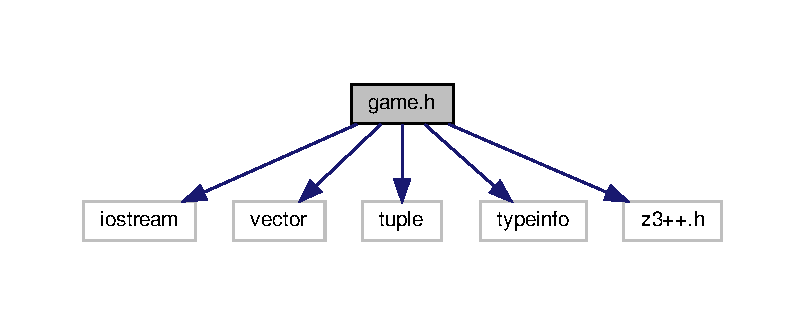
\includegraphics[width=350pt]{game_8h__incl}
\end{center}
\end{figure}
This graph shows which files directly or indirectly include this file\+:
\nopagebreak
\begin{figure}[H]
\begin{center}
\leavevmode
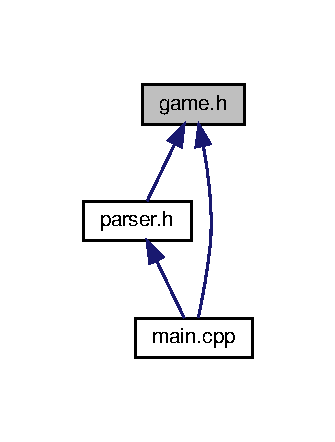
\includegraphics[width=161pt]{game_8h__dep__incl}
\end{center}
\end{figure}
\subsection*{Classes}
\begin{DoxyCompactItemize}
\item 
class \hyperlink{classGame}{Game}
\end{DoxyCompactItemize}


\subsection{Detailed Description}
Header for the game object.

The game object is used to encode a safety game. It stores initial vertices, safe vertices, player0 vertices, player1 vertices, edges, variables and additional expressions for the learner. \begin{DoxyAuthor}{Author}
Oliver Markgraf 
\end{DoxyAuthor}
\begin{DoxyDate}{Date}
August 14 
\end{DoxyDate}

\hypertarget{main_8cpp}{}\section{main.\+cpp File Reference}
\label{main_8cpp}\index{main.\+cpp@{main.\+cpp}}
{\ttfamily \#include $<$iostream$>$}\newline
{\ttfamily \#include $<$fstream$>$}\newline
{\ttfamily \#include $<$vector$>$}\newline
{\ttfamily \#include $<$string$>$}\newline
{\ttfamily \#include $<$set$>$}\newline
{\ttfamily \#include $<$map$>$}\newline
{\ttfamily \#include $<$iterator$>$}\newline
{\ttfamily \#include $<$typeinfo$>$}\newline
{\ttfamily \#include \char`\"{}z3++.\+h\char`\"{}}\newline
{\ttfamily \#include \char`\"{}parser.\+h\char`\"{}}\newline
{\ttfamily \#include \char`\"{}game.\+h\char`\"{}}\newline
{\ttfamily \#include \char`\"{}teacher.\+h\char`\"{}}\newline
{\ttfamily \#include $<$nlohmann/json.\+hpp$>$}\newline
{\ttfamily \#include $<$chrono$>$}\newline
Include dependency graph for main.\+cpp\+:
\nopagebreak
\begin{figure}[H]
\begin{center}
\leavevmode
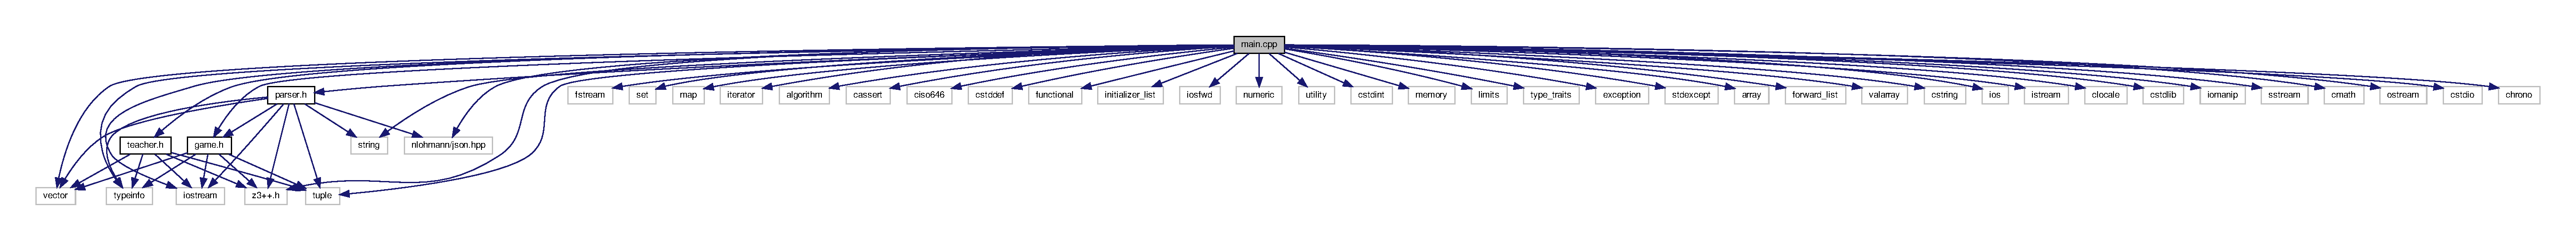
\includegraphics[width=350pt]{main_8cpp__incl}
\end{center}
\end{figure}
\subsection*{Classes}
\begin{DoxyCompactItemize}
\item 
struct \hyperlink{structCounterexample}{Counterexample}
\begin{DoxyCompactList}\small\item\em \hyperlink{structCounterexample}{Counterexample} struct to encode counterexamples. \end{DoxyCompactList}\end{DoxyCompactItemize}
\subsection*{Typedefs}
\begin{DoxyCompactItemize}
\item 
\mbox{\Hypertarget{main_8cpp_ab701e3ac61a85b337ec5c1abaad6742d}\label{main_8cpp_ab701e3ac61a85b337ec5c1abaad6742d}} 
using {\bfseries json} = nlohmann\+::json
\end{DoxyCompactItemize}
\subsection*{Functions}
\begin{DoxyCompactItemize}
\item 
z3\+::expr \hyperlink{main_8cpp_a05c829d51ea32790a877238ae39cddbe}{read\+\_\+json} (json \&j, std\+::map$<$ std\+::string, z3\+::expr $>$ \&variables, std\+::map$<$ std\+::string, z3\+::expr $>$ \&exprs\+\_\+map, int level, std\+::string \&tree)
\item 
void \hyperlink{main_8cpp_a0e97bf58e07b2914129e1455b405ae40}{prep} (std\+::vector$<$ std\+::string $>$ \&attributes)
\item 
void \hyperlink{main_8cpp_aac759501cf6c7895a70eecbef0226ae1}{write} ()
\item 
void \hyperlink{main_8cpp_a7f8b71f39cbfbfa39318854114f5223e}{store\+\_\+horn} (std\+::vector$<$ int $>$ horn)
\item 
void \hyperlink{main_8cpp_aac651fcf73c60a84961aadf71d3d9601}{eval\+\_\+exprs} (std\+::vector$<$ int $>$ \&ce, const z3\+::expr\+\_\+vector \&variables\+\_\+vector, const z3\+::expr\+\_\+vector \&exprs, const z3\+::expr\+\_\+vector \&expr\+\_\+vars)
\item 
int \hyperlink{main_8cpp_a05d3ee2c937a102a96c0f7bf43345582}{store} (\hyperlink{structCounterexample}{Counterexample} ce, const z3\+::expr\+\_\+vector \&variables\+\_\+vector, const z3\+::expr\+\_\+vector \&exprs, const z3\+::expr\+\_\+vector \&expr\+\_\+vars)
\item 
int \hyperlink{main_8cpp_ab16e639e29e2148cb8bbedab27c927ee}{create\+\_\+and\+\_\+store\+\_\+initial\+\_\+counterexample} (std\+::vector$<$ int $>$ \&ce, const z3\+::expr\+\_\+vector \&variables\+\_\+vector, const z3\+::expr\+\_\+vector \&exprs, const z3\+::expr\+\_\+vector \&expr\+\_\+vars)
\item 
int \hyperlink{main_8cpp_ad9cb78a282786d0e3c340d1eb442533f}{create\+\_\+and\+\_\+store\+\_\+safe\+\_\+counterexample} (std\+::vector$<$ int $>$ \&ce, const z3\+::expr\+\_\+vector \&variables\+\_\+vector, const z3\+::expr\+\_\+vector \&exprs, const z3\+::expr\+\_\+vector \&expr\+\_\+vars)
\item 
int \hyperlink{main_8cpp_a8f88348f60022c5218973949c1176b19}{create\+\_\+and\+\_\+store\+\_\+unclassified\+\_\+counterexample} (std\+::vector$<$ int $>$ \&ce, const z3\+::expr\+\_\+vector \&variables\+\_\+vector, const z3\+::expr\+\_\+vector \&exprs, const z3\+::expr\+\_\+vector \&expr\+\_\+vars)
\item 
bool \hyperlink{main_8cpp_aea111e2b2380b47fd98ae1112229e9aa}{create\+\_\+and\+\_\+store\+\_\+existential\+\_\+counterexample} (std\+::vector$<$ std\+::vector$<$ int $>$$>$ \&ce, const z3\+::expr\+\_\+vector \&variables\+\_\+vector, const z3\+::expr\+\_\+vector \&exprs, const z3\+::expr\+\_\+vector \&expr\+\_\+vars)
\item 
bool \hyperlink{main_8cpp_ac158554b7d2399f8855417c89b5d732f}{create\+\_\+and\+\_\+store\+\_\+universal\+\_\+counterexample} (std\+::vector$<$ std\+::vector$<$ int $>$$>$ \&ce, const z3\+::expr\+\_\+vector \&variables\+\_\+vector, const z3\+::expr\+\_\+vector \&exprs, const z3\+::expr\+\_\+vector \&expr\+\_\+vars)
\item 
bool \hyperlink{main_8cpp_a9f9117fc0c279c0486e7c621e6cf48a8}{initial\+\_\+check} (const z3\+::expr \&hypothesis, const z3\+::expr \&initial\+\_\+vertices, z3\+::context \&context, const z3\+::expr\+\_\+vector \&variables, const z3\+::expr\+\_\+vector \&exprs, const z3\+::expr\+\_\+vector \&expr\+\_\+vars)
\item 
bool \hyperlink{main_8cpp_a63731766047cbbe8b336311930e42455}{safe\+\_\+check} (const z3\+::expr \&hypothesis, const z3\+::expr \&safe\+\_\+vertices, z3\+::context \&context, const z3\+::expr\+\_\+vector \&variables, const z3\+::expr\+\_\+vector \&exprs, const z3\+::expr\+\_\+vector \&expr\+\_\+vars)
\item 
bool \hyperlink{main_8cpp_aef6432b1d800fa50de929258bf0cdce0}{ex\+\_\+check} (const z3\+::expr \&hypothesis, z3\+::expr \&hypothesis\+\_\+edge\+\_\+nodes, const z3\+::expr \&vertices, const z3\+::expr \&vertices\+\_\+dash, const z3\+::expr \&vertices\+\_\+player0, const z3\+::expr \&edges, z3\+::context \&context, const z3\+::expr\+\_\+vector \&all\+\_\+variables, const z3\+::expr\+\_\+vector \&variables, const z3\+::expr\+\_\+vector \&variables\+\_\+dash, const int \&n, const z3\+::expr\+\_\+vector \&exprs, const z3\+::expr\+\_\+vector \&expr\+\_\+vars)
\item 
bool \hyperlink{main_8cpp_a53a6fca0bec48e7ed06163689d83bc0a}{uni\+\_\+check} (const z3\+::expr \&hypothesis, z3\+::expr \&hypothesis\+\_\+edge\+\_\+nodes, const z3\+::expr \&vertices, const z3\+::expr \&vertices\+\_\+dash, const z3\+::expr \&vertices\+\_\+player1, const z3\+::expr \&edges, z3\+::context \&context, const z3\+::expr\+\_\+vector \&all\+\_\+variables, const z3\+::expr\+\_\+vector \&variables, const z3\+::expr\+\_\+vector \&variables\+\_\+dash, const int n, const z3\+::expr\+\_\+vector \&exprs, const z3\+::expr\+\_\+vector \&expr\+\_\+vars)
\item 
void \hyperlink{main_8cpp_ad05d3ac5d6fbd2a01301d0a2e69cf08b}{generate\+\_\+stats} (std\+::string \&result, \hyperlink{classGame}{Game} $\ast$\&game, int steps, std\+::vector$<$ double $>$ \&stats)
\item 
int \hyperlink{main_8cpp_a0ddf1224851353fc92bfbff6f499fa97}{main} (int argc, char $\ast$argv\mbox{[}$\,$\mbox{]})
\end{DoxyCompactItemize}
\subsection*{Variables}
\begin{DoxyCompactItemize}
\item 
\mbox{\Hypertarget{main_8cpp_ade4560be108f65d2a5c44be4f78afb99}\label{main_8cpp_ade4560be108f65d2a5c44be4f78afb99}} 
std\+::map$<$ \hyperlink{structCounterexample}{Counterexample}, int $>$ {\bfseries counterexample\+\_\+map}
\item 
\mbox{\Hypertarget{main_8cpp_aa0f8f2512327a68a51f0a2d4789b203f}\label{main_8cpp_aa0f8f2512327a68a51f0a2d4789b203f}} 
std\+::map$<$ int, \hyperlink{structCounterexample}{Counterexample} $>$ {\bfseries position\+\_\+map}
\item 
\mbox{\Hypertarget{main_8cpp_a0d0a2bbfb4cc99668a05c7cc7930a4c0}\label{main_8cpp_a0d0a2bbfb4cc99668a05c7cc7930a4c0}} 
std\+::vector$<$ \hyperlink{structCounterexample}{Counterexample} $>$ {\bfseries counterexample\+\_\+vector}
\item 
\mbox{\Hypertarget{main_8cpp_ae47c8bfae4b3046ecf040fafafb2df4e}\label{main_8cpp_ae47c8bfae4b3046ecf040fafafb2df4e}} 
std\+::vector$<$ std\+::vector$<$ int $>$ $>$ {\bfseries horn\+\_\+clauses}
\item 
\mbox{\Hypertarget{main_8cpp_ae67bd383e767098e5d69712ff4420610}\label{main_8cpp_ae67bd383e767098e5d69712ff4420610}} 
z3\+::context {\bfseries ctx}
\end{DoxyCompactItemize}


\subsection{Detailed Description}
Main file for learner and teacher interaction.

Implements the loop between learner and teacher and the communication between them. \begin{DoxyAuthor}{Author}
Oliver Markgraf 
\end{DoxyAuthor}
\begin{DoxyDate}{Date}
August 14 
\end{DoxyDate}


\subsection{Function Documentation}
\mbox{\Hypertarget{main_8cpp_aea111e2b2380b47fd98ae1112229e9aa}\label{main_8cpp_aea111e2b2380b47fd98ae1112229e9aa}} 
\index{main.\+cpp@{main.\+cpp}!create\+\_\+and\+\_\+store\+\_\+existential\+\_\+counterexample@{create\+\_\+and\+\_\+store\+\_\+existential\+\_\+counterexample}}
\index{create\+\_\+and\+\_\+store\+\_\+existential\+\_\+counterexample@{create\+\_\+and\+\_\+store\+\_\+existential\+\_\+counterexample}!main.\+cpp@{main.\+cpp}}
\subsubsection{\texorpdfstring{create\+\_\+and\+\_\+store\+\_\+existential\+\_\+counterexample()}{create\_and\_store\_existential\_counterexample()}}
{\footnotesize\ttfamily bool create\+\_\+and\+\_\+store\+\_\+existential\+\_\+counterexample (\begin{DoxyParamCaption}\item[{std\+::vector$<$ std\+::vector$<$ int $>$$>$ \&}]{ce,  }\item[{const z3\+::expr\+\_\+vector \&}]{variables\+\_\+vector,  }\item[{const z3\+::expr\+\_\+vector \&}]{exprs,  }\item[{const z3\+::expr\+\_\+vector \&}]{expr\+\_\+vars }\end{DoxyParamCaption})}

Method to create and store a counterexamples for the existential condition. calls \begin{DoxySeeAlso}{See also}
\hyperlink{main_8cpp_a8f88348f60022c5218973949c1176b19}{create\+\_\+and\+\_\+store\+\_\+unclassified\+\_\+counterexample}, to create an unclassified counterexample for each node and its successors. 
\end{DoxySeeAlso}

\begin{DoxyParams}{Parameters}
{\em ce} & -\/ data points of the counterexample with its successors, encoded as vector of int vectors \\
\hline
{\em variables\+\_\+vector} & -\/ variables as z3\+::expr \\
\hline
{\em exprs} & -\/ additional expressions for the learner \\
\hline
{\em expr\+\_\+vars} & -\/ additional expression variables for the learner \\
\hline
\end{DoxyParams}
\begin{DoxyReturn}{Returns}
returns true if the method was successful, false if it was unsucessful 
\end{DoxyReturn}
\mbox{\Hypertarget{main_8cpp_ab16e639e29e2148cb8bbedab27c927ee}\label{main_8cpp_ab16e639e29e2148cb8bbedab27c927ee}} 
\index{main.\+cpp@{main.\+cpp}!create\+\_\+and\+\_\+store\+\_\+initial\+\_\+counterexample@{create\+\_\+and\+\_\+store\+\_\+initial\+\_\+counterexample}}
\index{create\+\_\+and\+\_\+store\+\_\+initial\+\_\+counterexample@{create\+\_\+and\+\_\+store\+\_\+initial\+\_\+counterexample}!main.\+cpp@{main.\+cpp}}
\subsubsection{\texorpdfstring{create\+\_\+and\+\_\+store\+\_\+initial\+\_\+counterexample()}{create\_and\_store\_initial\_counterexample()}}
{\footnotesize\ttfamily int create\+\_\+and\+\_\+store\+\_\+initial\+\_\+counterexample (\begin{DoxyParamCaption}\item[{std\+::vector$<$ int $>$ \&}]{ce,  }\item[{const z3\+::expr\+\_\+vector \&}]{variables\+\_\+vector,  }\item[{const z3\+::expr\+\_\+vector \&}]{exprs,  }\item[{const z3\+::expr\+\_\+vector \&}]{expr\+\_\+vars }\end{DoxyParamCaption})}

Method to create and store a counterexample for the initial condition. Sets classification to 0. 
\begin{DoxyParams}{Parameters}
{\em ce} & -\/ data points of the counterexample, encoded as int vector \\
\hline
{\em variables\+\_\+vector} & -\/ variables as z3\+::expr \\
\hline
{\em exprs} & -\/ additional expressions for the learner \\
\hline
{\em expr\+\_\+vars} & -\/ additional expression variables for the learner \\
\hline
\end{DoxyParams}
\begin{DoxyReturn}{Returns}
returns the position of the stored counterexample, -\/1 if it was unsucessful 
\end{DoxyReturn}
\mbox{\Hypertarget{main_8cpp_ad9cb78a282786d0e3c340d1eb442533f}\label{main_8cpp_ad9cb78a282786d0e3c340d1eb442533f}} 
\index{main.\+cpp@{main.\+cpp}!create\+\_\+and\+\_\+store\+\_\+safe\+\_\+counterexample@{create\+\_\+and\+\_\+store\+\_\+safe\+\_\+counterexample}}
\index{create\+\_\+and\+\_\+store\+\_\+safe\+\_\+counterexample@{create\+\_\+and\+\_\+store\+\_\+safe\+\_\+counterexample}!main.\+cpp@{main.\+cpp}}
\subsubsection{\texorpdfstring{create\+\_\+and\+\_\+store\+\_\+safe\+\_\+counterexample()}{create\_and\_store\_safe\_counterexample()}}
{\footnotesize\ttfamily int create\+\_\+and\+\_\+store\+\_\+safe\+\_\+counterexample (\begin{DoxyParamCaption}\item[{std\+::vector$<$ int $>$ \&}]{ce,  }\item[{const z3\+::expr\+\_\+vector \&}]{variables\+\_\+vector,  }\item[{const z3\+::expr\+\_\+vector \&}]{exprs,  }\item[{const z3\+::expr\+\_\+vector \&}]{expr\+\_\+vars }\end{DoxyParamCaption})}

Method to create and store a counterexample for the safe condition. Sets classification to 1. 
\begin{DoxyParams}{Parameters}
{\em ce} & -\/ data points of the counterexample, encoded as int vector \\
\hline
{\em variables\+\_\+vector} & -\/ variables as z3\+::expr \\
\hline
{\em exprs} & -\/ additional expressions for the learner \\
\hline
{\em expr\+\_\+vars} & -\/ additional expression variables for the learner \\
\hline
\end{DoxyParams}
\begin{DoxyReturn}{Returns}
returns the position of the stored counterexample, -\/1 if it was unsucessful 
\end{DoxyReturn}
\mbox{\Hypertarget{main_8cpp_a8f88348f60022c5218973949c1176b19}\label{main_8cpp_a8f88348f60022c5218973949c1176b19}} 
\index{main.\+cpp@{main.\+cpp}!create\+\_\+and\+\_\+store\+\_\+unclassified\+\_\+counterexample@{create\+\_\+and\+\_\+store\+\_\+unclassified\+\_\+counterexample}}
\index{create\+\_\+and\+\_\+store\+\_\+unclassified\+\_\+counterexample@{create\+\_\+and\+\_\+store\+\_\+unclassified\+\_\+counterexample}!main.\+cpp@{main.\+cpp}}
\subsubsection{\texorpdfstring{create\+\_\+and\+\_\+store\+\_\+unclassified\+\_\+counterexample()}{create\_and\_store\_unclassified\_counterexample()}}
{\footnotesize\ttfamily int create\+\_\+and\+\_\+store\+\_\+unclassified\+\_\+counterexample (\begin{DoxyParamCaption}\item[{std\+::vector$<$ int $>$ \&}]{ce,  }\item[{const z3\+::expr\+\_\+vector \&}]{variables\+\_\+vector,  }\item[{const z3\+::expr\+\_\+vector \&}]{exprs,  }\item[{const z3\+::expr\+\_\+vector \&}]{expr\+\_\+vars }\end{DoxyParamCaption})}

Method to create and store a counterexample for the existential or universal condition. Sets classification to -\/1. 
\begin{DoxyParams}{Parameters}
{\em ce} & -\/ data points of the counterexample, encoded as int vector \\
\hline
{\em variables\+\_\+vector} & -\/ variables as z3\+::expr \\
\hline
{\em exprs} & -\/ additional expressions for the learner \\
\hline
{\em expr\+\_\+vars} & -\/ additional expression variables for the learner \\
\hline
\end{DoxyParams}
\begin{DoxyReturn}{Returns}
returns the position of the stored counterexample, -\/1 if it was unsucessful 
\end{DoxyReturn}
\mbox{\Hypertarget{main_8cpp_ac158554b7d2399f8855417c89b5d732f}\label{main_8cpp_ac158554b7d2399f8855417c89b5d732f}} 
\index{main.\+cpp@{main.\+cpp}!create\+\_\+and\+\_\+store\+\_\+universal\+\_\+counterexample@{create\+\_\+and\+\_\+store\+\_\+universal\+\_\+counterexample}}
\index{create\+\_\+and\+\_\+store\+\_\+universal\+\_\+counterexample@{create\+\_\+and\+\_\+store\+\_\+universal\+\_\+counterexample}!main.\+cpp@{main.\+cpp}}
\subsubsection{\texorpdfstring{create\+\_\+and\+\_\+store\+\_\+universal\+\_\+counterexample()}{create\_and\_store\_universal\_counterexample()}}
{\footnotesize\ttfamily bool create\+\_\+and\+\_\+store\+\_\+universal\+\_\+counterexample (\begin{DoxyParamCaption}\item[{std\+::vector$<$ std\+::vector$<$ int $>$$>$ \&}]{ce,  }\item[{const z3\+::expr\+\_\+vector \&}]{variables\+\_\+vector,  }\item[{const z3\+::expr\+\_\+vector \&}]{exprs,  }\item[{const z3\+::expr\+\_\+vector \&}]{expr\+\_\+vars }\end{DoxyParamCaption})}

Method to create and store a counterexamples for the universal condition. calls \begin{DoxySeeAlso}{See also}
\hyperlink{main_8cpp_a8f88348f60022c5218973949c1176b19}{create\+\_\+and\+\_\+store\+\_\+unclassified\+\_\+counterexample}, to create an unclassified counterexample for each node and its successors. 
\end{DoxySeeAlso}

\begin{DoxyParams}{Parameters}
{\em ce} & -\/ data points of the counterexample with its successors, encoded as vector of int vectors \\
\hline
{\em variables\+\_\+vector} & -\/ variables as z3\+::expr \\
\hline
{\em exprs} & -\/ additional expressions for the learner \\
\hline
{\em expr\+\_\+vars} & -\/ additional expression variables for the learner \\
\hline
\end{DoxyParams}
\begin{DoxyReturn}{Returns}
returns true if the method was successful, false if it was unsucessful 
\end{DoxyReturn}
\mbox{\Hypertarget{main_8cpp_aac651fcf73c60a84961aadf71d3d9601}\label{main_8cpp_aac651fcf73c60a84961aadf71d3d9601}} 
\index{main.\+cpp@{main.\+cpp}!eval\+\_\+exprs@{eval\+\_\+exprs}}
\index{eval\+\_\+exprs@{eval\+\_\+exprs}!main.\+cpp@{main.\+cpp}}
\subsubsection{\texorpdfstring{eval\+\_\+exprs()}{eval\_exprs()}}
{\footnotesize\ttfamily void eval\+\_\+exprs (\begin{DoxyParamCaption}\item[{std\+::vector$<$ int $>$ \&}]{ce,  }\item[{const z3\+::expr\+\_\+vector \&}]{variables\+\_\+vector,  }\item[{const z3\+::expr\+\_\+vector \&}]{exprs,  }\item[{const z3\+::expr\+\_\+vector \&}]{expr\+\_\+vars }\end{DoxyParamCaption})}

Method to evaluate the additional expressions give by the user. Adds the evaluation to the counterexample vector. 
\begin{DoxyParams}{Parameters}
{\em ce} & -\/ the counterexample vector, used to extend the counterexample \\
\hline
{\em variables\+\_\+vector} & -\/ variables, used to assign values to the counterexample \\
\hline
{\em exprs} & -\/ vector of the additional expressions \\
\hline
{\em expr\+\_\+vars} & -\/ variables used in the additional expressions \\
\hline
\end{DoxyParams}
\mbox{\Hypertarget{main_8cpp_aef6432b1d800fa50de929258bf0cdce0}\label{main_8cpp_aef6432b1d800fa50de929258bf0cdce0}} 
\index{main.\+cpp@{main.\+cpp}!ex\+\_\+check@{ex\+\_\+check}}
\index{ex\+\_\+check@{ex\+\_\+check}!main.\+cpp@{main.\+cpp}}
\subsubsection{\texorpdfstring{ex\+\_\+check()}{ex\_check()}}
{\footnotesize\ttfamily bool ex\+\_\+check (\begin{DoxyParamCaption}\item[{const z3\+::expr \&}]{hypothesis,  }\item[{z3\+::expr \&}]{hypothesis\+\_\+edge\+\_\+nodes,  }\item[{const z3\+::expr \&}]{vertices,  }\item[{const z3\+::expr \&}]{vertices\+\_\+dash,  }\item[{const z3\+::expr \&}]{vertices\+\_\+player0,  }\item[{const z3\+::expr \&}]{edges,  }\item[{z3\+::context \&}]{context,  }\item[{const z3\+::expr\+\_\+vector \&}]{all\+\_\+variables,  }\item[{const z3\+::expr\+\_\+vector \&}]{variables,  }\item[{const z3\+::expr\+\_\+vector \&}]{variables\+\_\+dash,  }\item[{const int \&}]{n,  }\item[{const z3\+::expr\+\_\+vector \&}]{exprs,  }\item[{const z3\+::expr\+\_\+vector \&}]{expr\+\_\+vars }\end{DoxyParamCaption})}

Method that calls the existential condition check in \hyperlink{teacher_8h}{teacher.\+h} 
\begin{DoxyParams}{Parameters}
{\em hypothesis} & -\/ hypothesis of a winning set encoded as z3\+::expr \\
\hline
{\em hypothesis\+\_\+edge\+\_\+nodes} & -\/ possible successors of the hypothesis after one step \\
\hline
{\em vertices} & -\/ vertices of the game graph \\
\hline
{\em vertices\+\_\+dash} & -\/ vertices encoded with the variables in the next step \\
\hline
{\em vertices\+\_\+player0} & -\/ vertices that are owned by player0 \\
\hline
{\em edges} & -\/ edges of the game graph \\
\hline
{\em context} & -\/ context to evaluate the expressions \\
\hline
{\em all\+\_\+variables} & -\/ variables and variables\+\_\+dash combined \\
\hline
{\em variables} & -\/ variables to get the value of each variable assigned \\
\hline
{\em variables\+\_\+dash} & -\/ variables in the next step \\
\hline
{\em n} & -\/ maximum number of successors \\
\hline
{\em exprs} & -\/ z3\+::expr\+\_\+vector of the additional expressions \\
\hline
{\em expr\+\_\+vars} & -\/ variables of the additional expressions \\
\hline
\end{DoxyParams}
\begin{DoxyReturn}{Returns}
true if counterexample was found, false if no counterexample was found 
\end{DoxyReturn}
\mbox{\Hypertarget{main_8cpp_ad05d3ac5d6fbd2a01301d0a2e69cf08b}\label{main_8cpp_ad05d3ac5d6fbd2a01301d0a2e69cf08b}} 
\index{main.\+cpp@{main.\+cpp}!generate\+\_\+stats@{generate\+\_\+stats}}
\index{generate\+\_\+stats@{generate\+\_\+stats}!main.\+cpp@{main.\+cpp}}
\subsubsection{\texorpdfstring{generate\+\_\+stats()}{generate\_stats()}}
{\footnotesize\ttfamily void generate\+\_\+stats (\begin{DoxyParamCaption}\item[{std\+::string \&}]{result,  }\item[{\hyperlink{classGame}{Game} $\ast$\&}]{game,  }\item[{int}]{steps,  }\item[{std\+::vector$<$ double $>$ \&}]{stats }\end{DoxyParamCaption})}

Method to generate overall stats of the safety game learning process. 
\begin{DoxyParams}{Parameters}
{\em result} & -\/ string to pass on the result and print it out later \\
\hline
{\em game} & -\/ game to access stats \\
\hline
{\em stats} & -\/ time statistics \\
\hline
\end{DoxyParams}
\mbox{\Hypertarget{main_8cpp_a9f9117fc0c279c0486e7c621e6cf48a8}\label{main_8cpp_a9f9117fc0c279c0486e7c621e6cf48a8}} 
\index{main.\+cpp@{main.\+cpp}!initial\+\_\+check@{initial\+\_\+check}}
\index{initial\+\_\+check@{initial\+\_\+check}!main.\+cpp@{main.\+cpp}}
\subsubsection{\texorpdfstring{initial\+\_\+check()}{initial\_check()}}
{\footnotesize\ttfamily bool initial\+\_\+check (\begin{DoxyParamCaption}\item[{const z3\+::expr \&}]{hypothesis,  }\item[{const z3\+::expr \&}]{initial\+\_\+vertices,  }\item[{z3\+::context \&}]{context,  }\item[{const z3\+::expr\+\_\+vector \&}]{variables,  }\item[{const z3\+::expr\+\_\+vector \&}]{exprs,  }\item[{const z3\+::expr\+\_\+vector \&}]{expr\+\_\+vars }\end{DoxyParamCaption})}

Method that calls the initial condition check in \hyperlink{teacher_8h}{teacher.\+h} 
\begin{DoxyParams}{Parameters}
{\em hypothesis} & -\/ hypothesis about the winning condition \\
\hline
{\em initial\+\_\+vertices} & -\/ initial vertices of the game graph \\
\hline
{\em context} & -\/ context to evaluate variables \\
\hline
{\em variables} & -\/ z3\+::expr\+\_\+vector of the variables used \\
\hline
{\em exprs} & -\/ z3\+::expr\+\_\+vector of the additional expressions \\
\hline
{\em expr\+\_\+vars} & -\/ variables of the additional expressions \\
\hline
\end{DoxyParams}
\begin{DoxyReturn}{Returns}
true if counterexample was found, false if no counterexample was found 
\end{DoxyReturn}
\mbox{\Hypertarget{main_8cpp_a0ddf1224851353fc92bfbff6f499fa97}\label{main_8cpp_a0ddf1224851353fc92bfbff6f499fa97}} 
\index{main.\+cpp@{main.\+cpp}!main@{main}}
\index{main@{main}!main.\+cpp@{main.\+cpp}}
\subsubsection{\texorpdfstring{main()}{main()}}
{\footnotesize\ttfamily int main (\begin{DoxyParamCaption}\item[{int}]{argc,  }\item[{char $\ast$}]{argv\mbox{[}$\,$\mbox{]} }\end{DoxyParamCaption})}

Main method that encodes the interaction between teacher and learner. 
\begin{DoxyParams}{Parameters}
{\em argc} & -\/ number of inputs, should be 2 \\
\hline
{\em argv} & -\/ argv\mbox{[}1\mbox{]}, should be the path to the input file \\
\hline
\end{DoxyParams}
\mbox{\Hypertarget{main_8cpp_a0e97bf58e07b2914129e1455b405ae40}\label{main_8cpp_a0e97bf58e07b2914129e1455b405ae40}} 
\index{main.\+cpp@{main.\+cpp}!prep@{prep}}
\index{prep@{prep}!main.\+cpp@{main.\+cpp}}
\subsubsection{\texorpdfstring{prep()}{prep()}}
{\footnotesize\ttfamily void prep (\begin{DoxyParamCaption}\item[{std\+::vector$<$ std\+::string $>$ \&}]{attributes }\end{DoxyParamCaption})}

Method to write attributes in a file for the learner. 
\begin{DoxyParams}{Parameters}
{\em attribute} & -\/ given attributes to write \\
\hline
\end{DoxyParams}
\mbox{\Hypertarget{main_8cpp_a05c829d51ea32790a877238ae39cddbe}\label{main_8cpp_a05c829d51ea32790a877238ae39cddbe}} 
\index{main.\+cpp@{main.\+cpp}!read\+\_\+json@{read\+\_\+json}}
\index{read\+\_\+json@{read\+\_\+json}!main.\+cpp@{main.\+cpp}}
\subsubsection{\texorpdfstring{read\+\_\+json()}{read\_json()}}
{\footnotesize\ttfamily z3\+::expr read\+\_\+json (\begin{DoxyParamCaption}\item[{json \&}]{j,  }\item[{std\+::map$<$ std\+::string, z3\+::expr $>$ \&}]{variables,  }\item[{std\+::map$<$ std\+::string, z3\+::expr $>$ \&}]{exprs\+\_\+map,  }\item[{int}]{level,  }\item[{std\+::string \&}]{tree }\end{DoxyParamCaption})}

Method to read a json file given by the learner.

Translates the json to a z3\+::expr. 
\begin{DoxyParams}{Parameters}
{\em variables} & -\/ a map to assign variable names to z3\+::expr variables \\
\hline
{\em exprs\+\_\+map} & -\/ a map to assign additional expression variables to z3\+::expr \\
\hline
{\em level} & -\/ the level the tree is at, used to print out the hypothesis \\
\hline
{\em tree} & -\/ string that is a output for the hypothesis \\
\hline
\end{DoxyParams}
\begin{DoxyReturn}{Returns}
Hypothesis from the learner encoded as z3\+::expr 
\end{DoxyReturn}
\mbox{\Hypertarget{main_8cpp_a63731766047cbbe8b336311930e42455}\label{main_8cpp_a63731766047cbbe8b336311930e42455}} 
\index{main.\+cpp@{main.\+cpp}!safe\+\_\+check@{safe\+\_\+check}}
\index{safe\+\_\+check@{safe\+\_\+check}!main.\+cpp@{main.\+cpp}}
\subsubsection{\texorpdfstring{safe\+\_\+check()}{safe\_check()}}
{\footnotesize\ttfamily bool safe\+\_\+check (\begin{DoxyParamCaption}\item[{const z3\+::expr \&}]{hypothesis,  }\item[{const z3\+::expr \&}]{safe\+\_\+vertices,  }\item[{z3\+::context \&}]{context,  }\item[{const z3\+::expr\+\_\+vector \&}]{variables,  }\item[{const z3\+::expr\+\_\+vector \&}]{exprs,  }\item[{const z3\+::expr\+\_\+vector \&}]{expr\+\_\+vars }\end{DoxyParamCaption})}

Method that calls the safe condition check in \hyperlink{teacher_8h}{teacher.\+h} 
\begin{DoxyParams}{Parameters}
{\em hypothesis} & -\/ hypothesis about the winning condition \\
\hline
{\em safe\+\_\+vertices} & -\/ safe vertices of the game graph \\
\hline
{\em context} & -\/ context to evaluate variables \\
\hline
{\em variables} & -\/ z3\+::expr\+\_\+vector of the variables used \\
\hline
{\em exprs} & -\/ z3\+::expr\+\_\+vector of the additional expressions \\
\hline
{\em expr\+\_\+vars} & -\/ variables of the additional expressions \\
\hline
\end{DoxyParams}
\begin{DoxyReturn}{Returns}
true if counterexample was found, false if no counterexample was found 
\end{DoxyReturn}
\mbox{\Hypertarget{main_8cpp_a05d3ee2c937a102a96c0f7bf43345582}\label{main_8cpp_a05d3ee2c937a102a96c0f7bf43345582}} 
\index{main.\+cpp@{main.\+cpp}!store@{store}}
\index{store@{store}!main.\+cpp@{main.\+cpp}}
\subsubsection{\texorpdfstring{store()}{store()}}
{\footnotesize\ttfamily int store (\begin{DoxyParamCaption}\item[{\hyperlink{structCounterexample}{Counterexample}}]{ce,  }\item[{const z3\+::expr\+\_\+vector \&}]{variables\+\_\+vector,  }\item[{const z3\+::expr\+\_\+vector \&}]{exprs,  }\item[{const z3\+::expr\+\_\+vector \&}]{expr\+\_\+vars }\end{DoxyParamCaption})}

Method to store counterexamples in a global field. 
\begin{DoxyParams}{Parameters}
{\em ce} & -\/ counterexample given as a \hyperlink{structCounterexample}{Counterexample} object \\
\hline
{\em variables\+\_\+vector} & -\/ passed on to evaluate the additional expressions \\
\hline
{\em exprs} & -\/ passed on to evaluate the additional expressions \\
\hline
{\em expr\+\_\+vars} & -\/ passed on to evaluate the additional expressions \\
\hline
\end{DoxyParams}
\begin{DoxyReturn}{Returns}
returns the position in the field, where the counterexample was written, -\/1 if the method was unsuccessful 
\end{DoxyReturn}
\mbox{\Hypertarget{main_8cpp_a7f8b71f39cbfbfa39318854114f5223e}\label{main_8cpp_a7f8b71f39cbfbfa39318854114f5223e}} 
\index{main.\+cpp@{main.\+cpp}!store\+\_\+horn@{store\+\_\+horn}}
\index{store\+\_\+horn@{store\+\_\+horn}!main.\+cpp@{main.\+cpp}}
\subsubsection{\texorpdfstring{store\+\_\+horn()}{store\_horn()}}
{\footnotesize\ttfamily void store\+\_\+horn (\begin{DoxyParamCaption}\item[{std\+::vector$<$ int $>$}]{horn }\end{DoxyParamCaption})}

Method to store horn clauses in a global field. \mbox{\Hypertarget{main_8cpp_a53a6fca0bec48e7ed06163689d83bc0a}\label{main_8cpp_a53a6fca0bec48e7ed06163689d83bc0a}} 
\index{main.\+cpp@{main.\+cpp}!uni\+\_\+check@{uni\+\_\+check}}
\index{uni\+\_\+check@{uni\+\_\+check}!main.\+cpp@{main.\+cpp}}
\subsubsection{\texorpdfstring{uni\+\_\+check()}{uni\_check()}}
{\footnotesize\ttfamily bool uni\+\_\+check (\begin{DoxyParamCaption}\item[{const z3\+::expr \&}]{hypothesis,  }\item[{z3\+::expr \&}]{hypothesis\+\_\+edge\+\_\+nodes,  }\item[{const z3\+::expr \&}]{vertices,  }\item[{const z3\+::expr \&}]{vertices\+\_\+dash,  }\item[{const z3\+::expr \&}]{vertices\+\_\+player1,  }\item[{const z3\+::expr \&}]{edges,  }\item[{z3\+::context \&}]{context,  }\item[{const z3\+::expr\+\_\+vector \&}]{all\+\_\+variables,  }\item[{const z3\+::expr\+\_\+vector \&}]{variables,  }\item[{const z3\+::expr\+\_\+vector \&}]{variables\+\_\+dash,  }\item[{const int}]{n,  }\item[{const z3\+::expr\+\_\+vector \&}]{exprs,  }\item[{const z3\+::expr\+\_\+vector \&}]{expr\+\_\+vars }\end{DoxyParamCaption})}

Method that calls the universal condition check in \hyperlink{teacher_8h}{teacher.\+h} 
\begin{DoxyParams}{Parameters}
{\em hypothesis} & -\/ hypothesis of a winning set encoded as z3\+::expr \\
\hline
{\em hypothesis\+\_\+edge\+\_\+nodes} & -\/ possible successors of the hypothesis after one step \\
\hline
{\em vertices} & -\/ vertices of the game graph \\
\hline
{\em vertices\+\_\+dash} & -\/ vertices encoded with the variables in the next step \\
\hline
{\em vertices\+\_\+player1} & -\/ vertices that are owned by player1 \\
\hline
{\em edges} & -\/ edges of the game graph \\
\hline
{\em context} & -\/ context to evaluate the expressions \\
\hline
{\em all\+\_\+variables} & -\/ variables and variables\+\_\+dash combined \\
\hline
{\em variables} & -\/ variables to get the value of each variable assigned \\
\hline
{\em variables\+\_\+dash} & -\/ variables in the next step \\
\hline
{\em n} & -\/ maximum number of successors \\
\hline
{\em exprs} & -\/ z3\+::expr\+\_\+vector of the additional expressions \\
\hline
{\em expr\+\_\+vars} & -\/ variables of the additional expressions \\
\hline
\end{DoxyParams}
\begin{DoxyReturn}{Returns}
true if counterexample was found, false if no counterexample was found 
\end{DoxyReturn}
\mbox{\Hypertarget{main_8cpp_aac759501cf6c7895a70eecbef0226ae1}\label{main_8cpp_aac759501cf6c7895a70eecbef0226ae1}} 
\index{main.\+cpp@{main.\+cpp}!write@{write}}
\index{write@{write}!main.\+cpp@{main.\+cpp}}
\subsubsection{\texorpdfstring{write()}{write()}}
{\footnotesize\ttfamily void write (\begin{DoxyParamCaption}{ }\end{DoxyParamCaption})}

Method to write counterexamples for the learner to a file. 
\hypertarget{teacher_8h}{}\section{teacher.\+h File Reference}
\label{teacher_8h}\index{teacher.\+h@{teacher.\+h}}
{\ttfamily \#include $<$iostream$>$}\newline
{\ttfamily \#include $<$vector$>$}\newline
{\ttfamily \#include $<$tuple$>$}\newline
{\ttfamily \#include $<$typeinfo$>$}\newline
{\ttfamily \#include \char`\"{}z3++.\+h\char`\"{}}\newline
Include dependency graph for teacher.\+h\+:
\nopagebreak
\begin{figure}[H]
\begin{center}
\leavevmode
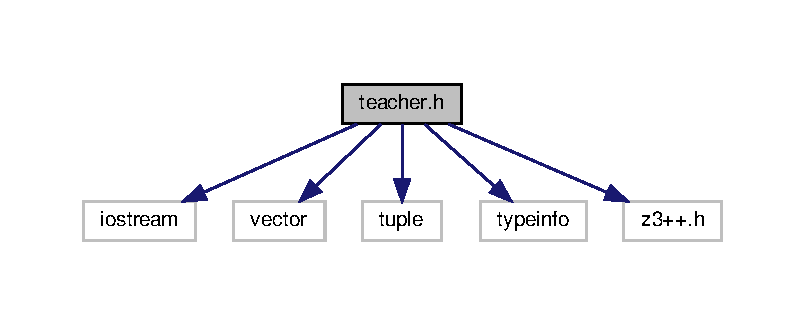
\includegraphics[width=350pt]{teacher_8h__incl}
\end{center}
\end{figure}
This graph shows which files directly or indirectly include this file\+:
\nopagebreak
\begin{figure}[H]
\begin{center}
\leavevmode
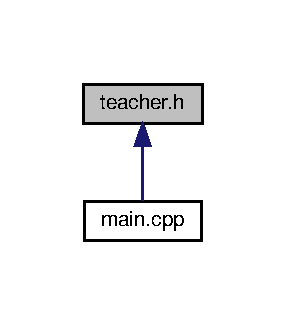
\includegraphics[width=137pt]{teacher_8h__dep__incl}
\end{center}
\end{figure}
\subsection*{Functions}
\begin{DoxyCompactItemize}
\item 
std\+::vector$<$ int $>$ \hyperlink{teacher_8h_aec1fd0b948385829532e05caf2ce9fa6}{check\+\_\+initial\+\_\+condition} (const z3\+::expr \&hypothesis, const z3\+::expr \&initial\+\_\+vertices, z3\+::context \&context, const z3\+::expr\+\_\+vector \&variables)
\item 
std\+::vector$<$ int $>$ \hyperlink{teacher_8h_aeabe39d27d05ea0bda7d0481df52541b}{check\+\_\+safe\+\_\+condition} (const z3\+::expr \&hypothesis, const z3\+::expr \&safe\+\_\+vertices, z3\+::context \&context, const z3\+::expr\+\_\+vector \&variables)
\item 
std\+::vector$<$ std\+::vector$<$ int $>$ $>$ \hyperlink{teacher_8h_a9217d55403f5e487bf7ac97a728e7b25}{build\+\_\+counterexample} (const z3\+::expr \&counterexample, const std\+::vector$<$ int $>$ \&start, const z3\+::expr \&edges, z3\+::context \&context, const z3\+::expr\+\_\+vector \&variables, const z3\+::expr\+\_\+vector \&variables\+\_\+dash, const z3\+::expr\+\_\+vector \&all\+\_\+variables, const int n)
\item 
std\+::vector$<$ std\+::vector$<$ int $>$ $>$ \hyperlink{teacher_8h_a3acaa31b9de19512fb734e356a54af7b}{existential\+\_\+check} (const z3\+::expr \&hypothesis, z3\+::expr \&hypothesis\+\_\+edge\+\_\+nodes, const z3\+::expr \&vertices, const z3\+::expr \&vertices\+\_\+dash, const z3\+::expr \&vertices\+\_\+player0, const z3\+::expr \&edges, z3\+::context \&context, const z3\+::expr\+\_\+vector \&all\+\_\+variables, const z3\+::expr\+\_\+vector \&variables, const z3\+::expr\+\_\+vector \&variables\+\_\+dash, const int \&n)
\item 
std\+::vector$<$ std\+::vector$<$ int $>$ $>$ \hyperlink{teacher_8h_a9c2ae867f683c54913e6e6059bbdee2c}{universal\+\_\+check} (const z3\+::expr \&hypothesis, z3\+::expr \&hypothesis\+\_\+edge\+\_\+nodes, const z3\+::expr \&vertices, const z3\+::expr \&vertices\+\_\+dash, const z3\+::expr \&vertices\+\_\+player1, const z3\+::expr \&edges, z3\+::context \&context, const z3\+::expr\+\_\+vector \&all\+\_\+variables, const z3\+::expr\+\_\+vector \&variables, const z3\+::expr\+\_\+vector \&variables\+\_\+dash, const int n)
\end{DoxyCompactItemize}


\subsection{Detailed Description}
Header for the teacher.

This file has methods to implement a teacher such as check conditions that are required to hold for a winning set. \begin{DoxyAuthor}{Author}
Oliver Markgraf 
\end{DoxyAuthor}
\begin{DoxyDate}{Date}
August 14 
\end{DoxyDate}


\subsection{Function Documentation}
\mbox{\Hypertarget{teacher_8h_a9217d55403f5e487bf7ac97a728e7b25}\label{teacher_8h_a9217d55403f5e487bf7ac97a728e7b25}} 
\index{teacher.\+h@{teacher.\+h}!build\+\_\+counterexample@{build\+\_\+counterexample}}
\index{build\+\_\+counterexample@{build\+\_\+counterexample}!teacher.\+h@{teacher.\+h}}
\subsubsection{\texorpdfstring{build\+\_\+counterexample()}{build\_counterexample()}}
{\footnotesize\ttfamily std\+::vector$<$std\+::vector$<$int$>$ $>$ build\+\_\+counterexample (\begin{DoxyParamCaption}\item[{const z3\+::expr \&}]{counterexample,  }\item[{const std\+::vector$<$ int $>$ \&}]{start,  }\item[{const z3\+::expr \&}]{edges,  }\item[{z3\+::context \&}]{context,  }\item[{const z3\+::expr\+\_\+vector \&}]{variables,  }\item[{const z3\+::expr\+\_\+vector \&}]{variables\+\_\+dash,  }\item[{const z3\+::expr\+\_\+vector \&}]{all\+\_\+variables,  }\item[{const int}]{n }\end{DoxyParamCaption})}

Method to build a transform a counterexample from z3\+::expr to a vector of int vectors. Used for existential and universal counterexamples.


\begin{DoxyParams}{Parameters}
{\em counterexample} & -\/ counterexample of the hypothesis encoded as z3\+::expr \\
\hline
{\em start} & -\/ This is the counterexample node. \\
\hline
{\em edges} & -\/ edges of the game graph \\
\hline
{\em context} & -\/ context to evaluate the expressions \\
\hline
{\em variables} & -\/ variables to get the value of each variable assigned \\
\hline
{\em variables\+\_\+dash} & -\/ variables in the next step \\
\hline
{\em all\+\_\+variables} & -\/ variables and variables\+\_\+dash combined \\
\hline
{\em n} & -\/ maximum number of successors \\
\hline
\end{DoxyParams}
\begin{DoxyReturn}{Returns}
Returns a counterexample as a horn clause. First vector is left side, rest of the vectors are the right side. 
\end{DoxyReturn}
\mbox{\Hypertarget{teacher_8h_aec1fd0b948385829532e05caf2ce9fa6}\label{teacher_8h_aec1fd0b948385829532e05caf2ce9fa6}} 
\index{teacher.\+h@{teacher.\+h}!check\+\_\+initial\+\_\+condition@{check\+\_\+initial\+\_\+condition}}
\index{check\+\_\+initial\+\_\+condition@{check\+\_\+initial\+\_\+condition}!teacher.\+h@{teacher.\+h}}
\subsubsection{\texorpdfstring{check\+\_\+initial\+\_\+condition()}{check\_initial\_condition()}}
{\footnotesize\ttfamily std\+::vector$<$int$>$ check\+\_\+initial\+\_\+condition (\begin{DoxyParamCaption}\item[{const z3\+::expr \&}]{hypothesis,  }\item[{const z3\+::expr \&}]{initial\+\_\+vertices,  }\item[{z3\+::context \&}]{context,  }\item[{const z3\+::expr\+\_\+vector \&}]{variables }\end{DoxyParamCaption})}

Checks the initial condition for a hypothesis of a safety game. I ⊆ W 
\begin{DoxyParams}{Parameters}
{\em hypothesis} & -\/ hypothesis about the winning set W \\
\hline
{\em initial\+\_\+vertices} & -\/ initial vertices encodeded as z3\+::expr \\
\hline
{\em context} & -\/ context to evaluate the expressions \\
\hline
{\em variables} & -\/ variables to get the value of each variable assigned \\
\hline
\end{DoxyParams}
\begin{DoxyReturn}{Returns}
The counterexample, encoded as a int vector. 
\end{DoxyReturn}
\mbox{\Hypertarget{teacher_8h_aeabe39d27d05ea0bda7d0481df52541b}\label{teacher_8h_aeabe39d27d05ea0bda7d0481df52541b}} 
\index{teacher.\+h@{teacher.\+h}!check\+\_\+safe\+\_\+condition@{check\+\_\+safe\+\_\+condition}}
\index{check\+\_\+safe\+\_\+condition@{check\+\_\+safe\+\_\+condition}!teacher.\+h@{teacher.\+h}}
\subsubsection{\texorpdfstring{check\+\_\+safe\+\_\+condition()}{check\_safe\_condition()}}
{\footnotesize\ttfamily std\+::vector$<$int$>$ check\+\_\+safe\+\_\+condition (\begin{DoxyParamCaption}\item[{const z3\+::expr \&}]{hypothesis,  }\item[{const z3\+::expr \&}]{safe\+\_\+vertices,  }\item[{z3\+::context \&}]{context,  }\item[{const z3\+::expr\+\_\+vector \&}]{variables }\end{DoxyParamCaption})}

Checks the initial condition for a hypothesis of a safety game. W ⊆ F 
\begin{DoxyParams}{Parameters}
{\em hypothesis} & -\/ hypothesis about the winning set W \\
\hline
{\em safe\+\_\+vertices} & -\/ safe vertices encodeded as z3\+::expr \\
\hline
{\em context} & -\/ context to evaluate the expressions \\
\hline
{\em variables} & -\/ variables to get the value of each variable assigned \\
\hline
\end{DoxyParams}
\begin{DoxyReturn}{Returns}
The counterexample, encoded as a int vector. 
\end{DoxyReturn}
\mbox{\Hypertarget{teacher_8h_a3acaa31b9de19512fb734e356a54af7b}\label{teacher_8h_a3acaa31b9de19512fb734e356a54af7b}} 
\index{teacher.\+h@{teacher.\+h}!existential\+\_\+check@{existential\+\_\+check}}
\index{existential\+\_\+check@{existential\+\_\+check}!teacher.\+h@{teacher.\+h}}
\subsubsection{\texorpdfstring{existential\+\_\+check()}{existential\_check()}}
{\footnotesize\ttfamily std\+::vector$<$std\+::vector$<$int$>$ $>$ existential\+\_\+check (\begin{DoxyParamCaption}\item[{const z3\+::expr \&}]{hypothesis,  }\item[{z3\+::expr \&}]{hypothesis\+\_\+edge\+\_\+nodes,  }\item[{const z3\+::expr \&}]{vertices,  }\item[{const z3\+::expr \&}]{vertices\+\_\+dash,  }\item[{const z3\+::expr \&}]{vertices\+\_\+player0,  }\item[{const z3\+::expr \&}]{edges,  }\item[{z3\+::context \&}]{context,  }\item[{const z3\+::expr\+\_\+vector \&}]{all\+\_\+variables,  }\item[{const z3\+::expr\+\_\+vector \&}]{variables,  }\item[{const z3\+::expr\+\_\+vector \&}]{variables\+\_\+dash,  }\item[{const int \&}]{n }\end{DoxyParamCaption})}

Method to find a existential counterexample in a hypothesis.


\begin{DoxyParams}{Parameters}
{\em hypothesis} & -\/ hypothesis of a winning set encoded as z3\+::expr \\
\hline
{\em hypothesis\+\_\+edge\+\_\+nodes} & -\/ possible successors of the hypothesis after one step \\
\hline
{\em vertices} & -\/ vertices of the game graph \\
\hline
{\em vertices\+\_\+dash} & -\/ vertices encoded with the variables in the next step \\
\hline
{\em vertices\+\_\+player0} & -\/ vertices that are owned by player0 \\
\hline
{\em edges} & -\/ edges of the game graph \\
\hline
{\em context} & -\/ context to evaluate the expressions \\
\hline
{\em all\+\_\+variables} & -\/ variables and variables\+\_\+dash combined \\
\hline
{\em variables} & -\/ variables to get the value of each variable assigned \\
\hline
{\em variables\+\_\+dash} & -\/ variables in the next step \\
\hline
{\em n} & -\/ maximum number of successors \\
\hline
\end{DoxyParams}
\begin{DoxyReturn}{Returns}
Returns a counterexample as a horn clause. First vector is left side, rest of the vectors are the right side. 
\end{DoxyReturn}
\mbox{\Hypertarget{teacher_8h_a9c2ae867f683c54913e6e6059bbdee2c}\label{teacher_8h_a9c2ae867f683c54913e6e6059bbdee2c}} 
\index{teacher.\+h@{teacher.\+h}!universal\+\_\+check@{universal\+\_\+check}}
\index{universal\+\_\+check@{universal\+\_\+check}!teacher.\+h@{teacher.\+h}}
\subsubsection{\texorpdfstring{universal\+\_\+check()}{universal\_check()}}
{\footnotesize\ttfamily std\+::vector$<$std\+::vector$<$int$>$ $>$ universal\+\_\+check (\begin{DoxyParamCaption}\item[{const z3\+::expr \&}]{hypothesis,  }\item[{z3\+::expr \&}]{hypothesis\+\_\+edge\+\_\+nodes,  }\item[{const z3\+::expr \&}]{vertices,  }\item[{const z3\+::expr \&}]{vertices\+\_\+dash,  }\item[{const z3\+::expr \&}]{vertices\+\_\+player1,  }\item[{const z3\+::expr \&}]{edges,  }\item[{z3\+::context \&}]{context,  }\item[{const z3\+::expr\+\_\+vector \&}]{all\+\_\+variables,  }\item[{const z3\+::expr\+\_\+vector \&}]{variables,  }\item[{const z3\+::expr\+\_\+vector \&}]{variables\+\_\+dash,  }\item[{const int}]{n }\end{DoxyParamCaption})}

Method to find a existential counterexample in a hypothesis.


\begin{DoxyParams}{Parameters}
{\em hypothesis} & -\/ hypothesis of a winning set encoded as z3\+::expr \\
\hline
{\em hypothesis\+\_\+edge\+\_\+nodes} & -\/ possible successors of the hypothesis after one step \\
\hline
{\em vertices} & -\/ vertices of the game graph \\
\hline
{\em vertices\+\_\+dash} & -\/ vertices encoded with the variables in the next step \\
\hline
{\em vertices\+\_\+player1} & -\/ vertices that are owned by player1 \\
\hline
{\em edges} & -\/ edges of the game graph \\
\hline
{\em context} & -\/ context to evaluate the expressions \\
\hline
{\em all\+\_\+variables} & -\/ variables and variables\+\_\+dash combined \\
\hline
{\em variables} & -\/ variables to get the value of each variable assigned \\
\hline
{\em variables\+\_\+dash} & -\/ variables in the next step \\
\hline
{\em n} & -\/ maximum number of successors \\
\hline
\end{DoxyParams}
\begin{DoxyReturn}{Returns}
Returns a counterexample as a horn clause. First vector is left side, rest of the vectors are the right side. 
\end{DoxyReturn}

%--- End generated contents ---

% Index
\backmatter
\newpage
\phantomsection
\clearemptydoublepage
\addcontentsline{toc}{chapter}{Index}
\printindex

\end{document}
